\documentclass{standalone}


\usepackage{tikz}
\usetikzlibrary{automata, positioning}

\begin{document}
    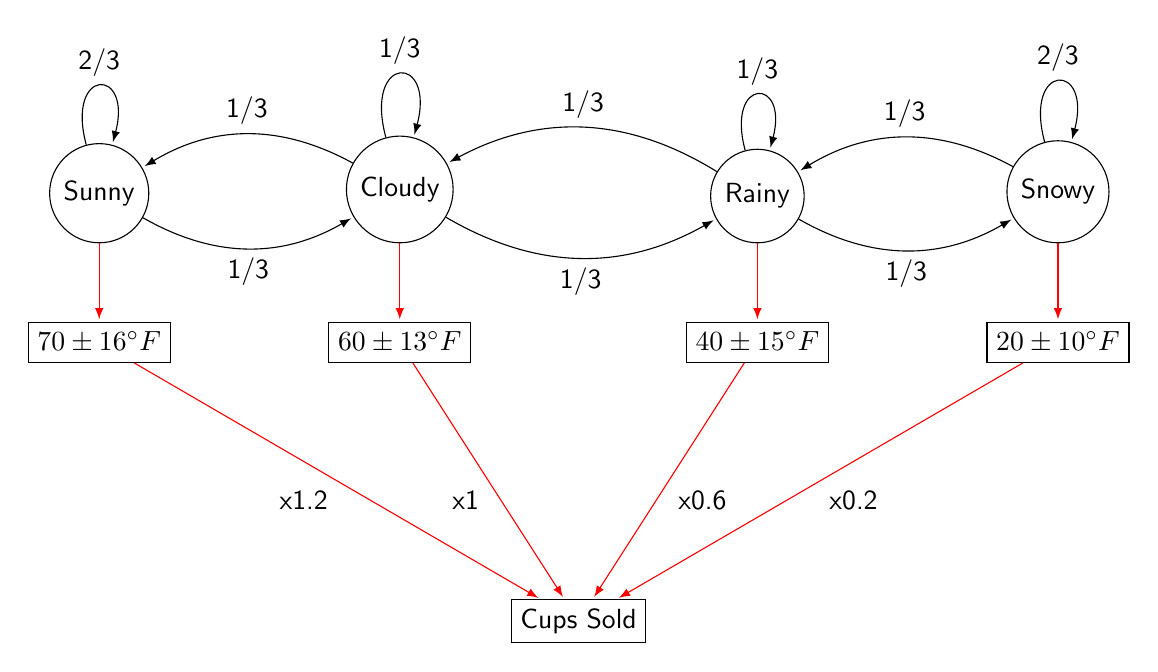
\begin{tikzpicture}[font=\sffamily]

     \tikzstyle{block} = [draw, rectangle]

    % Cups Sold
    \node [block] (cups) {Cups Sold};

    % Add the Temperatures
    \node [block, above left=3cm and 0.5cm of cups] (ct) {$60 \pm 13^{\circ}F$};
    \node [block, above right=3cm and 0.5cm of cups] (rt) {$40 \pm 15^{\circ}F$};
    \node [block, left=2cm of ct] (st) {$70 \pm 16^{\circ}F$};
    \node [block, right=2cm of rt] (nt) {$20 \pm 10^{\circ}F$};

    % Add the states
    \node[state, above=of st] (s) {Sunny};
    \node[state, above=of ct] (c) {Cloudy};
    \node[state, above=of rt] (r) {Rainy};
    \node[state, above=of nt] (n) {Snowy};


    % Connect the states with arrows
    \draw[every loop,
          auto=right,
          >=latex]

        % Sunny
        (s) edge[bend right, auto=right]  node {1/3} (c)
        (s) edge[loop above]             node {2/3} (s)
        (s) edge[draw=red] node {} (st)
        (st) edge[draw=red] node {x1.2} (cups)

        % Cloudy
        (c) edge[bend right, auto=right]  node {1/3} (s)
        (c) edge[bend right, auto=right]  node {1/3} (r)
        (c) edge[loop above]             node {1/3} (c)
        (c) edge[draw=red] node {} (ct)
        (ct) edge[draw=red] node {x1} (cups)

        % Rainy
        (r) edge[bend right, auto=right]  node {1/3} (c)
        (r) edge[bend right, auto=right]  node {1/3} (n)
        (r) edge[loop above]             node {1/3} (r)
        (r) edge[draw=red] node {} (rt)
        (rt) edge[draw=red,auto=left] node {x0.6} (cups)

        % Snowy
        (n) edge[bend right, auto=right]  node {1/3} (r)
        (n) edge[loop above]             node {2/3} (n)
        (n) edge[draw=red] node {} (nt)
        (nt) edge[draw=red,auto=left] node {x0.2} (cups);


   \end{tikzpicture}
\end{document}
